
\documentclass[11pt]{article}
\usepackage[a4paper,margin=1in]{geometry}
\usepackage{amsmath,amssymb}
\usepackage{graphicx}
\usepackage[dvipsnames]{xcolor}
\usepackage{hyperref}
\usepackage{enumitem}
\usepackage{tabularx}
\usepackage{longtable}
\usepackage{booktabs}
\usepackage[most]{tcolorbox}
\usepackage{titlesec}
\usepackage{xurl}
\usepackage{fancyhdr}
\usepackage{setspace}
\usepackage{tikz}
\usetikzlibrary{positioning,arrows.meta}
\usepackage[T1]{fontenc}
\usepackage{lmodern}
\setlength{\parindent}{0pt}
\setlength{\parskip}{8pt}
\setlength{\headheight}{14pt}
\setstretch{1.12}
\setlist[itemize]{leftmargin=1.5em, nosep}
\setlist[enumerate]{leftmargin=1.5em, nosep}
\providecommand{\tightlist}{\setlength{\itemsep}{0pt}\setlength{\parskip}{0pt}}
\hypersetup{colorlinks=true,linkcolor=MidnightBlue,urlcolor=MidnightBlue}
\pagestyle{fancy}
\raggedbottom
\fancyhf{}
\rhead{\thepage}
\renewcommand{\headrulewidth}{0pt}
\renewcommand{\footrulewidth}{0pt}
\titleformat{\section}{\Large\bfseries\color{MidnightBlue}}{\thesection}{0.6em}{}
\titleformat{\subsection}{\bfseries}{}{0em}{}


\begin{document}

\begin{center}\LARGE\bfseries Block 4 Tutorial -- Bayesian Networks, Exact Inference, Temporal Models, MDP Planning, DDNs, and POMDPs\end{center}

\begin{center}\large Block 4 Tutorial\end{center}

\begin{tcolorbox}[colback=MidnightBlue!4,colframe=MidnightBlue,title={Session Overview},fonttitle=\bfseries,breakable]
\textbf{Session objective:} Consolidate the full Block 4 reasoning arc from uncertain belief to hidden-state planning using longer-form tutorial problems.

\textbf{Timing target (min):} 86

\textbf{Topic anchors:} bayesian network; exact inference; dynamic bayesian network; markov decision process; dynamic decision network; partially observable markov decision process

\textbf{Padlet board:} \url{https://padlet.com/qmul/b4-tutorial-6a1s440grh9uprtn}
\end{tcolorbox}

\section*{Exercises}

\begin{tcolorbox}[colback=white,colframe=MidnightBlue,title={Q1 BN Structure and Assumptions},fonttitle=\bfseries,breakable]
\begin{center}
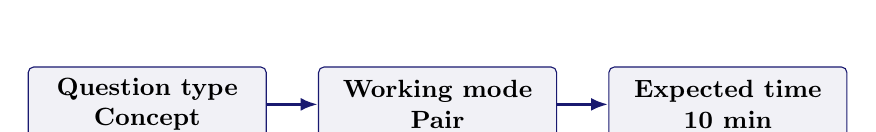
\begin{tikzpicture}[
node distance=0.65cm,
box/.style={draw=MidnightBlue, rounded corners=2pt, minimum height=0.95cm, align=center, font=\small\bfseries, fill=MidnightBlue!6, text width=0.23\linewidth},
arrow/.style={-{Latex[length=2.2mm]}, very thick, MidnightBlue}
]
\node[box] (type) {Question type\\Concept};
\node[box, right=of type] (mode) {Working mode\\Pair};
\node[box, right=of mode] (time) {Expected time\\10 min};
\draw[arrow] (type) -- (mode);
\draw[arrow] (mode) -- (time);
\end{tikzpicture}
\end{center}

{\large\bfseries\color{MidnightBlue} Prompt}\par\medskip
A student says, ``Once I draw a Bayesian network, the hard part is over because the edges already tell me the exact probabilities.'' Explain why this statement is wrong, and include one point about graph structure, one about CPTs, and one about model assumptions.

{\large\bfseries\color{MidnightBlue} Task details}\par\medskip
\begin{itemize}\item \textbf{Type:} concept
\item \textbf{Mode:} pair
\item \textbf{Time:} 10 min
\item \textbf{Deliverable:} short explanation
\item \textbf{Assessment focus:} explain what a BN structure commits you to
\item \textbf{Expected length:} 4 bullets\end{itemize}

{\large\bfseries\color{MidnightBlue} How to submit}\par\medskip
Post one pair Padlet comment with four short bullets.

{\large\bfseries\color{MidnightBlue} Discussion in class}\par\medskip
Which mistake is more dangerous: a wrong edge or a wrong number?

{\large\bfseries\color{MidnightBlue} Why this helps}\par\medskip
Helps with BN explanation questions in a fresh setting.

{\large\bfseries\color{MidnightBlue} References}\par\medskip
\begin{itemize}\item Russell \& Norvig (2021) AIMA 4e, Ch.12-13, pp.385-460
\item Poole \& Mackworth (2023) 3e, Ch.9, pp.375-458\end{itemize}
\end{tcolorbox}

\begin{tcolorbox}[colback=white,colframe=MidnightBlue,title={Q2 Dependence Reasoning},fonttitle=\bfseries,breakable]
\begin{center}
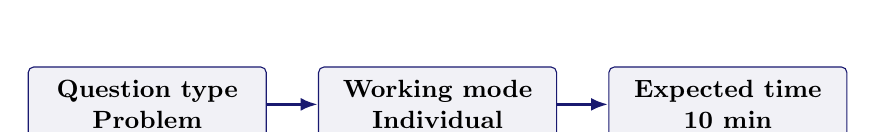
\begin{tikzpicture}[
node distance=0.65cm,
box/.style={draw=MidnightBlue, rounded corners=2pt, minimum height=0.95cm, align=center, font=\small\bfseries, fill=MidnightBlue!6, text width=0.23\linewidth},
arrow/.style={-{Latex[length=2.2mm]}, very thick, MidnightBlue}
]
\node[box] (type) {Question type\\Problem};
\node[box, right=of type] (mode) {Working mode\\Individual};
\node[box, right=of mode] (time) {Expected time\\10 min};
\draw[arrow] (type) -- (mode);
\draw[arrow] (mode) -- (time);
\end{tikzpicture}
\end{center}

{\large\bfseries\color{MidnightBlue} Prompt}\par\medskip
Decide whether the end variables are dependent or independent in these three patterns, both before and after the middle variable is observed: (1) Weather -\textgreater{} Picnic -\textgreater{} Mood, (2) ExamStress \textless- Deadlines -\textgreater{} SleepLoss, (3) Malware -\textgreater{} Alert \textless- BenignSoftware.

{\large\bfseries\color{MidnightBlue} Task details}\par\medskip
\begin{itemize}\item \textbf{Type:} problem
\item \textbf{Mode:} individual
\item \textbf{Time:} 10 min
\item \textbf{Deliverable:} dependence judgements
\item \textbf{Assessment focus:} reason about open and blocked paths in named scenarios
\item \textbf{Expected length:} 6 answers\end{itemize}

{\large\bfseries\color{MidnightBlue} How to submit}\par\medskip
Post your own Padlet comment with six answers and one short reason for each pattern.

{\large\bfseries\color{MidnightBlue} Discussion in class}\par\medskip
Which pattern changed most when the middle node was observed?

{\large\bfseries\color{MidnightBlue} Why this helps}\par\medskip
Strengthens conditional-independence reasoning in a fresh setting.

{\large\bfseries\color{MidnightBlue} References}\par\medskip
\begin{itemize}\item Russell \& Norvig (2021) AIMA 4e, Ch.12-13, pp.385-460
\item Poole \& Mackworth (2023) 3e, Ch.9, pp.375-458\end{itemize}
\end{tcolorbox}

\begin{tcolorbox}[colback=white,colframe=MidnightBlue,title={Q3 Exact Inference Practice},fonttitle=\bfseries,breakable]
\begin{center}
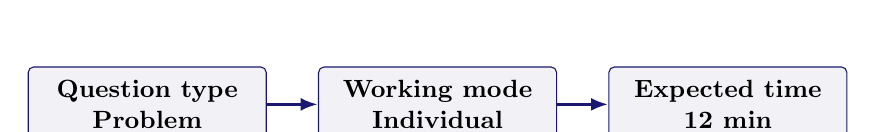
\begin{tikzpicture}[
node distance=0.65cm,
box/.style={draw=MidnightBlue, rounded corners=2pt, minimum height=0.95cm, align=center, font=\small\bfseries, fill=MidnightBlue!6, text width=0.23\linewidth},
arrow/.style={-{Latex[length=2.2mm]}, very thick, MidnightBlue}
]
\node[box] (type) {Question type\\Problem};
\node[box, right=of type] (mode) {Working mode\\Individual};
\node[box, right=of mode] (time) {Expected time\\12 min};
\draw[arrow] (type) -- (mode);
\draw[arrow] (mode) -- (time);
\end{tikzpicture}
\end{center}

{\large\bfseries\color{MidnightBlue} Prompt}\par\medskip
In the Alarm network, compute P(Earthquake=true \textbar{} JohnCalls=true, MaryCalls=false) using enumeration. You may reuse the standard Alarm network CPT values from class. Show the two unnormalized scores and the normalization step clearly.

\begin{tcolorbox}[colback=ForestGreen!5,colframe=ForestGreen,title={Formula reminder},fonttitle=\bfseries,breakable]
\[
P(X \mid e)=\alpha \, P(X,e)
\]
\[
P(X,e)=\sum_{h} P(X,e,h)
\]
\textbf{Use this when you must compute two unnormalised scores and then normalise.}
\end{tcolorbox}

{\large\bfseries\color{MidnightBlue} Task details}\par\medskip
\begin{itemize}\item \textbf{Type:} problem
\item \textbf{Mode:} individual
\item \textbf{Time:} 12 min
\item \textbf{Deliverable:} worked calculation
\item \textbf{Assessment focus:} perform enumeration with normalization on a small BN query
\item \textbf{Expected length:} 5 lines\end{itemize}

{\large\bfseries\color{MidnightBlue} How to submit}\par\medskip
Post your own Padlet comment with the two scores, the normalization step, and the final posterior.

{\large\bfseries\color{MidnightBlue} Discussion in class}\par\medskip
Which hidden variable contributes most to the repeated work?

{\large\bfseries\color{MidnightBlue} Why this helps}\par\medskip
Gives exact-inference practice with a different query focus.

{\large\bfseries\color{MidnightBlue} References}\par\medskip
\begin{itemize}\item Russell \& Norvig (2021) AIMA 4e, Ch.13, pp.412-460
\item Poole \& Mackworth (2023) 3e, Ch.9, pp.375-458\end{itemize}
\end{tcolorbox}

\begin{tcolorbox}[colback=white,colframe=MidnightBlue,title={Q4 Variable Elimination and Complexity},fonttitle=\bfseries,breakable]
\begin{center}
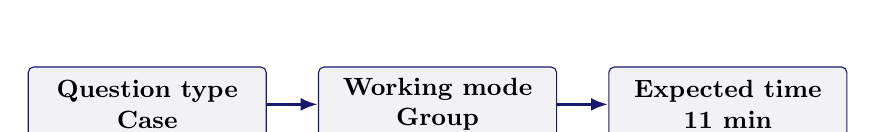
\begin{tikzpicture}[
node distance=0.65cm,
box/.style={draw=MidnightBlue, rounded corners=2pt, minimum height=0.95cm, align=center, font=\small\bfseries, fill=MidnightBlue!6, text width=0.23\linewidth},
arrow/.style={-{Latex[length=2.2mm]}, very thick, MidnightBlue}
]
\node[box] (type) {Question type\\Case};
\node[box, right=of type] (mode) {Working mode\\Group};
\node[box, right=of mode] (time) {Expected time\\11 min};
\draw[arrow] (type) -- (mode);
\draw[arrow] (mode) -- (time);
\end{tikzpicture}
\end{center}

{\large\bfseries\color{MidnightBlue} Prompt}\par\medskip
A medical BN has edges Season -\textgreater{} Pollen, Season -\textgreater{} Influenza, Pollen -\textgreater{} HayFever, Influenza -\textgreater{} Fever, and both HayFever and Influenza -\textgreater{} Sneezing. For the query P(Influenza \textbar{} Sneezing=true), propose an elimination order and explain where factor growth becomes dangerous.

{\large\bfseries\color{MidnightBlue} Task details}\par\medskip
\begin{itemize}\item \textbf{Type:} case
\item \textbf{Mode:} group
\item \textbf{Time:} 11 min
\item \textbf{Deliverable:} elimination memo
\item \textbf{Assessment focus:} choose a sensible elimination order and explain the risk of a bad one
\item \textbf{Expected length:} order + 3 bullets\end{itemize}

{\large\bfseries\color{MidnightBlue} How to submit}\par\medskip
Post one group Padlet comment with the order and three bullets on factor growth.

{\large\bfseries\color{MidnightBlue} Discussion in class}\par\medskip
Which variable feels harmless but becomes expensive if eliminated too early?

{\large\bfseries\color{MidnightBlue} Why this helps}\par\medskip
Builds VE intuition on a different network structure.

{\large\bfseries\color{MidnightBlue} References}\par\medskip
\begin{itemize}\item Russell \& Norvig (2021) AIMA 4e, Ch.13, pp.412-460
\item Poole \& Mackworth (2023) 3e, Ch.9, pp.375-458\end{itemize}
\end{tcolorbox}

\begin{tcolorbox}[colback=white,colframe=MidnightBlue,title={Q5 Temporal Model Choice},fonttitle=\bfseries,breakable]
\begin{center}
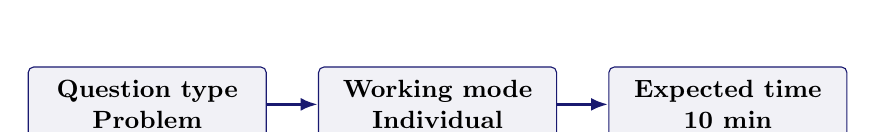
\begin{tikzpicture}[
node distance=0.65cm,
box/.style={draw=MidnightBlue, rounded corners=2pt, minimum height=0.95cm, align=center, font=\small\bfseries, fill=MidnightBlue!6, text width=0.23\linewidth},
arrow/.style={-{Latex[length=2.2mm]}, very thick, MidnightBlue}
]
\node[box] (type) {Question type\\Problem};
\node[box, right=of type] (mode) {Working mode\\Individual};
\node[box, right=of mode] (time) {Expected time\\10 min};
\draw[arrow] (type) -- (mode);
\draw[arrow] (mode) -- (time);
\end{tikzpicture}
\end{center}

{\large\bfseries\color{MidnightBlue} Prompt}\par\medskip
Match each scenario to the most suitable temporal model: (1) temperature tracking with continuous noisy sensor values, (2) umbrella-and-rain style discrete hidden weather, (3) a robot with position, battery state, and sensor faults evolving together. Choose from hidden Markov model, Kalman filter, and dynamic Bayesian network, and explain why.

{\large\bfseries\color{MidnightBlue} Task details}\par\medskip
\begin{itemize}\item \textbf{Type:} problem
\item \textbf{Mode:} individual
\item \textbf{Time:} 10 min
\item \textbf{Deliverable:} model-choice explanation
\item \textbf{Assessment focus:} choose between HMM, Kalman filter, and DBN
\item \textbf{Expected length:} 3 labelled answers\end{itemize}

{\large\bfseries\color{MidnightBlue} How to submit}\par\medskip
Post your own Padlet comment with three choices and one short reason each.

{\large\bfseries\color{MidnightBlue} Discussion in class}\par\medskip
Which feature most strongly forces the DBN choice?

{\large\bfseries\color{MidnightBlue} Why this helps}\par\medskip
Helps with temporal model selection under different assumptions.

{\large\bfseries\color{MidnightBlue} References}\par\medskip
\begin{itemize}\item Russell \& Norvig (2021) AIMA 4e, Ch.14, pp.461-499
\item Poole \& Mackworth (2023) 3e, Ch.9, pp.375-458\end{itemize}
\end{tcolorbox}

\begin{tcolorbox}[colback=white,colframe=MidnightBlue,title={Q6 Planning Model Choice},fonttitle=\bfseries,breakable]
\begin{center}
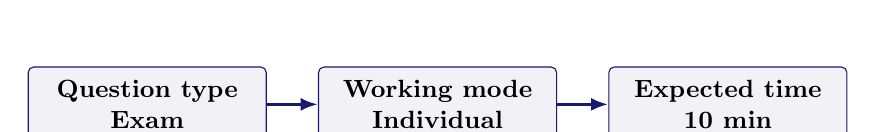
\begin{tikzpicture}[
node distance=0.65cm,
box/.style={draw=MidnightBlue, rounded corners=2pt, minimum height=0.95cm, align=center, font=\small\bfseries, fill=MidnightBlue!6, text width=0.23\linewidth},
arrow/.style={-{Latex[length=2.2mm]}, very thick, MidnightBlue}
]
\node[box] (type) {Question type\\Exam};
\node[box, right=of type] (mode) {Working mode\\Individual};
\node[box, right=of mode] (time) {Expected time\\10 min};
\draw[arrow] (type) -- (mode);
\draw[arrow] (mode) -- (time);
\end{tikzpicture}
\end{center}

{\large\bfseries\color{MidnightBlue} Prompt}\par\medskip
A classmate makes these model choices: (1) ``Use a partially observable Markov decision process for a one-off insurance purchase decision,'' (2) ``Use a decision network for a warehouse robot that moves every minute in a fully observed map,'' and (3) ``Use a Markov decision process for a wildfire drone when smoke hides the true fire boundary.'' For each case, say whether the choice is correct. If it is wrong, replace it with a better model and give one reason.

{\large\bfseries\color{MidnightBlue} Task details}\par\medskip
\begin{itemize}\item \textbf{Type:} exam
\item \textbf{Mode:} individual
\item \textbf{Time:} 10 min
\item \textbf{Deliverable:} critique-and-correct note
\item \textbf{Assessment focus:} diagnose wrong planning-model choices by checking repetition, observability, and uncertainty
\item \textbf{Expected length:} 3 short corrections\end{itemize}

{\large\bfseries\color{MidnightBlue} How to submit}\par\medskip
Post your own Padlet comment with three labelled judgements and one reason for each.

{\large\bfseries\color{MidnightBlue} Discussion in class}\par\medskip
Which mistake comes from ignoring repeated decisions, and which mistake comes from ignoring hidden state?

{\large\bfseries\color{MidnightBlue} Why this helps}\par\medskip
Strengthens planning-model discrimination through a critique-and-correct task.

{\large\bfseries\color{MidnightBlue} References}\par\medskip
\begin{itemize}\item Russell \& Norvig (2021) AIMA 4e, Ch.16-18
\item Poole \& Mackworth (2023) 3e, Ch.12, pp.517-582\end{itemize}
\end{tcolorbox}

\begin{tcolorbox}[colback=white,colframe=MidnightBlue,title={Q7 DDN and POMDP Synthesis Case},fonttitle=\bfseries,breakable]
\begin{center}
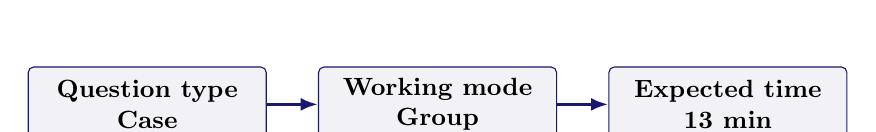
\begin{tikzpicture}[
node distance=0.65cm,
box/.style={draw=MidnightBlue, rounded corners=2pt, minimum height=0.95cm, align=center, font=\small\bfseries, fill=MidnightBlue!6, text width=0.23\linewidth},
arrow/.style={-{Latex[length=2.2mm]}, very thick, MidnightBlue}
]
\node[box] (type) {Question type\\Case};
\node[box, right=of type] (mode) {Working mode\\Group};
\node[box, right=of mode] (time) {Expected time\\13 min};
\draw[arrow] (type) -- (mode);
\draw[arrow] (mode) -- (time);
\end{tikzpicture}
\end{center}

{\large\bfseries\color{MidnightBlue} Prompt}\par\medskip
Design a small incident-response pipeline for either healthcare or cybersecurity. Your design must include: a temporal belief update, one decision step, one utility consideration, one place where the true state is partly hidden, and one human oversight gate.

\begin{tcolorbox}[colback=ForestGreen!5,colframe=ForestGreen,title={Formula reminder},fonttitle=\bfseries,breakable]
\[
b'(s')=\alpha \, P(o \mid s') \sum_{s} P(s' \mid s,a)\,b(s)
\]
\textbf{Use this when the task asks for a filtered or belief-state update.}
\end{tcolorbox}

{\large\bfseries\color{MidnightBlue} Task details}\par\medskip
\begin{itemize}\item \textbf{Type:} case
\item \textbf{Mode:} group
\item \textbf{Time:} 13 min
\item \textbf{Deliverable:} mini workflow
\item \textbf{Assessment focus:} connect belief, action, and human oversight in one applied pipeline
\item \textbf{Expected length:} 6 bullets\end{itemize}

{\large\bfseries\color{MidnightBlue} How to submit}\par\medskip
Post one group Padlet comment with six bullets covering those five required parts plus one domain-specific detail.

{\large\bfseries\color{MidnightBlue} Discussion in class}\par\medskip
Which part of the workflow carries the greatest uncertainty burden?

{\large\bfseries\color{MidnightBlue} Why this helps}\par\medskip
Helps with capstone synthesis thinking in a fresh applied scenario.

{\large\bfseries\color{MidnightBlue} References}\par\medskip
\begin{itemize}\item Russell \& Norvig (2021) AIMA 4e, Ch.17-18
\item Poole \& Mackworth (2023) 3e, Ch.12-13, pp.517-608\end{itemize}
\end{tcolorbox}

\begin{tcolorbox}[colback=white,colframe=MidnightBlue,title={Q8 Stretch Cross-Block Reflection},fonttitle=\bfseries,breakable]
\begin{center}
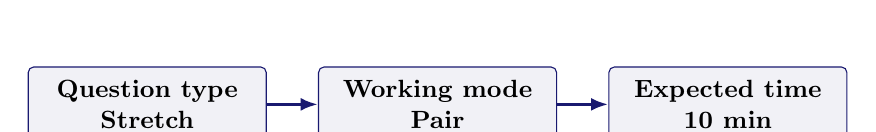
\begin{tikzpicture}[
node distance=0.65cm,
box/.style={draw=MidnightBlue, rounded corners=2pt, minimum height=0.95cm, align=center, font=\small\bfseries, fill=MidnightBlue!6, text width=0.23\linewidth},
arrow/.style={-{Latex[length=2.2mm]}, very thick, MidnightBlue}
]
\node[box] (type) {Question type\\Stretch};
\node[box, right=of type] (mode) {Working mode\\Pair};
\node[box, right=of mode] (time) {Expected time\\10 min};
\draw[arrow] (type) -- (mode);
\draw[arrow] (mode) -- (time);
\end{tikzpicture}
\end{center}

{\large\bfseries\color{MidnightBlue} Prompt}\par\medskip
Choose one agent setting from the module, such as healthcare assistant, cybersecurity response, or autonomous driving. Explain which Block 4 models are most useful there and which one would be overkill.

{\large\bfseries\color{MidnightBlue} Task details}\par\medskip
\begin{itemize}\item \textbf{Type:} stretch
\item \textbf{Mode:} pair
\item \textbf{Time:} 10 min
\item \textbf{Deliverable:} short reflection
\item \textbf{Assessment focus:} connect Block 4 uncertainty tools to agent-system design choices
\item \textbf{Expected length:} 5 bullets\end{itemize}

{\large\bfseries\color{MidnightBlue} How to submit}\par\medskip
Post one pair Padlet comment with five bullets naming the useful models and the one that would be overkill.

{\large\bfseries\color{MidnightBlue} Discussion in class}\par\medskip
When is a more expressive uncertainty model not worth the complexity?

{\large\bfseries\color{MidnightBlue} Why this helps}\par\medskip
Helps students choose models intelligently rather than collecting jargon.

{\large\bfseries\color{MidnightBlue} References}\par\medskip
\begin{itemize}\item Russell \& Norvig (2021) AIMA 4e, Ch.12-18
\item Poole \& Mackworth (2023) 3e, Ch.9 and Ch.12-13, pp.375-608\end{itemize}
\end{tcolorbox}

\section*{Submission Instructions}

Use the seeded Padlet posts for Q1--Q8. Q2, Q3, Q5, and Q6 are individual. Q1 and Q8 are pair tasks. Q4 and Q7 should be one joint group comment. Start each comment with your names or group label.

\section*{Whole-Class Debrief Prompts}

\begin{itemize}
\tightlist
\item
  Which Block 4 model still feels the most abstract after the lecture week?
\item
  Which tutorial problem felt closest to exam preparation without turning into an exam clone?
\item
  Where does full observability break most clearly across the whole block?
\end{itemize}

\section*{Exam Transfer Note (Day-Level)}

This tutorial consolidates Bayesian networks, exact inference, temporal reasoning, MDP planning, DDNs, and POMDPs in an exam-preparation style across new application settings.

\end{document}
